\documentclass[%
 reprint,
%superscriptaddress,
%groupedaddress,
%unsortedaddress,
%runinaddress,
%frontmatterverbose, 
%preprint,
%preprintnumbers,
%nofootinbib,
%nobibnotes,
%bibnotes,
 amsmath,amssymb,
 aps,
%pra,
%prb,
%rmp,
%prstab,
%prstper,
%floatfix,
]{revtex4-2}
\usepackage[utf8]{inputenc}
%\usepackage{amsmath}
\usepackage{color}
%\usepackage{amsmath}
%\usepackage{mathtools}
%\usepackage{bm}
%\usepackage{amsfonts}
%\usepackage{dcolumn}
%\usepackage{bbold}
%\usepackage{soul}
%\usepackage[dvipsnames]{xcolor}
%\usepackage{amssymb}
\usepackage[breaklinks=true,colorlinks,citecolor=red,linkcolor=blue,urlcolor=blue]{hyperref}
\usepackage{graphicx}
%\newcommand{\RN}[1]{%
%  \textup{\uppercase\expandafter{\romannumeral#1}}%
%}
\def\be{\begin{equation}}
\def\ee{\end{equation}}
\def \bea{\begin{eqnarray}}
\def \eea{\end{eqnarray}}
\def \nn{\nonumber}
%\renewcommand*{\thesection}{\Roman{section}}
%\renewcommand*{\thesubsection}{\Alph{subsection}}
%\renewcommand*{\thesubsubsection}{\roman{subsubsection}}
%\newcommand{\tc}[1]{\textcolor{red}{#1}}
%\usepackage{appendix}

\usepackage{mathtools}
%\usepackage{stfloats}
\begin{document}
\title{EE798K Assignment 4: Speach Detection Model}
%\author{Imran Ahamed}
%\email{imranad@iitk.ac.in}
%	\affiliation{Department of Electrical Engineering, Indian Institute of Technology, Kanpur 208016, India}

\author{Chinmay Hiran Pillai}
%\email{chinmay20@iitk.ac.in}
%\thanks{\\ $\dagger \dagger$ Corresponding author}	
\affiliation{200298}
\date{\today}% It is always \today, today,

\begin{abstract}
    The paper explores a speech recognition model that utilises Mel-Frequency Cepstral Coefficients (MFCCs)
    and Deep Neural Networks (DNNs) to detect speech from audio signals. It first outlines the architecture
    and features of the proposed model, then delves into the critical requirements necessary for real-time
    processing. The discussion then extends to potential challenges faced during implementation and provides
    strategies to mitigate these issues.
    %Triangular lattices are a promising platform for various magnetic phases and potential applications. Recently, room-temperature ferromagnetism was observed in triangular, few-layer CrTe crystals. In this study, we predict that monolayer CrTe, obtained by cleaving the [002] surface, is dynamically stable, shows half-metallicity with a large half-metal gap, and orders ferromagnetically with a high transition temperature. Our Monte Carlo simulations indicate that the monolayer CrTe has a high magnetic transition temperature of about 400 K. Additionally, we show that monolayer CrTe exhibits significant in-plane magnetocrystalline anisotropy energy. We have explored the ferroelectric characteristics of the monolayer owing to its broken inversion symmetry and buckled geometry hosting permanent electric dipole. Finally, we explored the polarization-induced tunability of anomalous Hall response due to band gap modulation. This makes it a promising material for spintronics and device applications. 
\end{abstract}

\maketitle

%\tableofcontents

\section{Introduction}
Mel-Frequency Cepstral Coefficients (MFCCs) have played a vital role towards in speech recognition
as they are crucial features that efficiently represent the power spectrum of audio
signals, serving as a pivotal component in the development of effective ASR systems \cite{huang2001spoken}.
Utilisation of Deep Neural Networks (DNNs) have also contributed heavily towards their advancement due to
their ability to learn complex features really well \cite{hinton2012deep}. \\

MFCCs serve as a reliable feature extractor, capturing the essential phenotic characteristics of the acoustic
signal, while DNNs offer robust pattern recognition capabilities, allowing the system to understand and
interpret these features accurately.

\section{Method Description}
The model involves first splitting the audio into short-time frames based on window size (w) and
hop size (h). We then need to classify each frame as containing speach or not, i.e run binary classification over
them. We utilise Deep Neural Networks (DNN) to classify the frames because of DNNs’ ability to handle
complex mappings between acoustic signals and phonetic classifications more effectively, thereby
enhancing the performance of ASR systems \cite{hinton2012deep}.\\

For the input for the classification, we need to provide the network with features that capture that phonemes
unique to speech which can be utilised to classify them. For this we use MFCCs since they capture the features
specific to speech and phonemes.\\

For even better performance, we will also provide the first and second differences of the MFCCs
($\Delta$MFCCs and $\Delta^2$MFCCs) in order to capture the features corresponding to how the MFCCs and
hence the phenomes are changing thoughout the audio. This should give the DNN more relevant information
to compute more accurate results. Since the number of MFCCs used are genrally small, calculating the
their first and second differences won't be relatively computationally expensive either.\\

\begin{figure}
    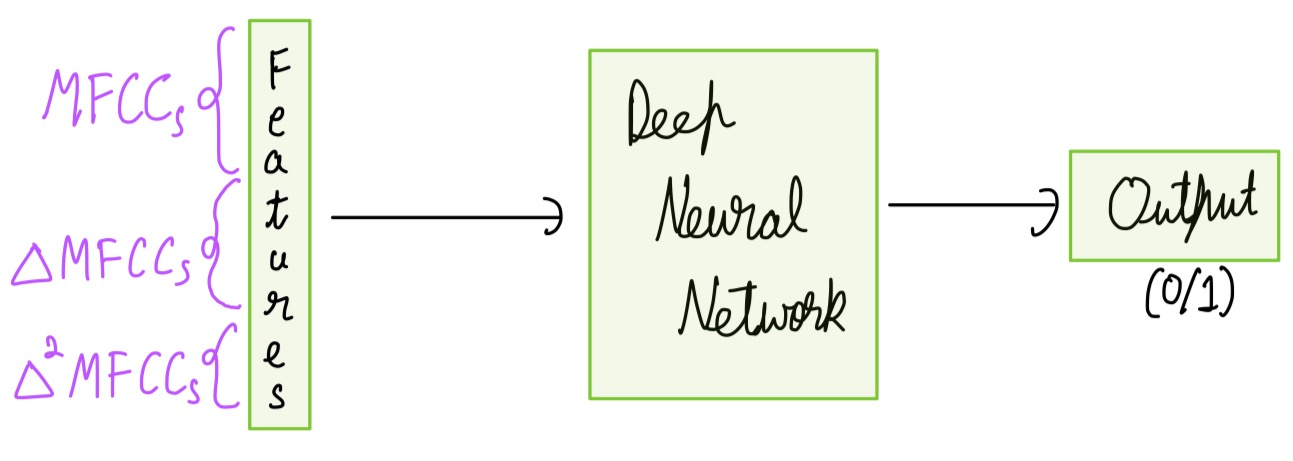
\includegraphics[scale=0.2]{Model.jpeg}
    \caption{Model for classifying each frame}
\end{figure}

\vspace{-8mm}

Once every frame has been classified as containing speech or not (1/0), we can find the start and end times
of speech using the following code,

\begin{figure}[h]
    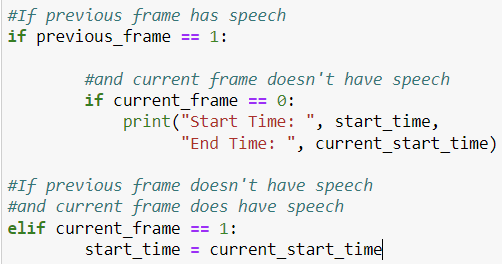
\includegraphics[scale=0.8]{StartEndCode.png}
    \caption{Code to run on every frame for finding start and end times}
\end{figure}

\vspace{-1mm}

where, "current start time" is the starting time for the current frame and "current frame" and "previous frame"
are the values outputted by the DNN (0/1) for the current and previous frame respectively.

\section{Discussion}
\vspace{-3mm}
\subsection{Real-Time Computation}
\vspace{-5mm}
For real-time computation we need to ensure that the execution time for processing the audio data till a
particular time is less than or equal to the particular time, i.e (number of windows processed at any current
time * Time required for processing 1 window $<=$ Current time)

%\vspace{-3mm}

\begin{equation}
    ( floor(\frac{t-w}{h}) + 1 ) * T <= t
\end{equation}

where,
\null\hfill T = Time required for processing 1 window \\
\null\hfill t = current time\\
\null\hfill w = window size\\
\null\hfill h = hop size

If the condition without the floor is satisfied, the above condition is also satisfied since the floor of a
number is less than or equal to the number. Then the condition for real-time computation become,

\begin{gather}
    (\frac{t-w}{h} + 1) * T <= t \\
    \implies \frac{t*T}{h} + ( 1 - \frac{w}{h} ) * T - t <= 0 \\
    \implies t *(\frac{T}{h} - 1) <= T * (\frac{w}{h} - 1)
\end{gather}

Since we maintain window size to be greater than the hop size, making $\frac{w}{h} > 1$,
we can observe that the RHS of the equation is positive. Since $t > 0$, the condition for satisfying
the equation for any $\frac{w}{h}$ ratio is making $( \frac{T}{h} - 1 ) <= 0$. Only then will the condition
satisfy $\forall w > h$.\\

Hence, for real-time computation, we require,

\begin{gather}
    \frac{T}{h} <= 1 \\
    \implies \mathbf{T <= h}
\end{gather}

Therefore, for real-time computation, we require the time required by the algorithm to process 1 window to be
less than the hop size of the spectrum. We hence need to choose our DNNs architecture and hop size
(and hence window size) carefully in order to enable real-time processing.

\vspace{-3mm}

\subsection{Gaps in Speech}
\vspace{-3mm}
Pauses are a common occurance during speech and we need our model to be capable of recognising them as parts
of the ongoing speech instead of classifying them as a break in speech. We can achieve this by optimizing
our window size to be bigger than the duration of a typical pause in speech but keeping it small enough to
achieve good precision.


\subsection{Hyperparameters}
The hyperparameters for the system are:

\begin{enumerate}
    \item Hop Size (h): Optimize for real-time computing as mention above
    \item Window Size (w): Optimize for presion, accuracy and computation time as mentioned above
    \item Architecture of the DNN: Optimise for accuracy while maintaining enough speed for real-time processing
    \item Number of MFCCs: Optimise for accuracy
    \item Learning Rate of DNN: Optimise for convergence to global minima of DNN's loss function
\end{enumerate}

%We need to optimize each of them for achiving the model's peak performance.


\section{Applications}
There are many application for Speech Detection, especially one which is fast enough for
real-time processing. Some of the apllications are \cite{juang2005automatic}:

\begin{enumerate}
    \item \textbf{Virtual Assistants}: Virtual assistants use ASR to convert user voice commands into text, enabling user-device interaction through natural language.
          %\item \textbf{Dictation Systems}: ASR is commonly used to convert spoken language into written text for documentation purposes.
    \item \textbf{Accessibility Tools}: ASR can be crucial for developing tools and technologies to assist individuals with disabilities.
    \item \textbf{In-Vehicle Voice Controlled Systems}: In-vehicle systems employ ASR to allow drivers to control navigation, music, and calls using voice commands, promoting hands-free operation.
          %\item \textbf{Healthcare Documentation}: Medical professionals utilize ASR to transcribe patient interactions and notes, reducing manual documentation workload.
\end{enumerate}




\section{Conclusion}
The paper explored a model for speech detection using MFCCs and DNNs. We then delved into the model's requirments
for real-time processing, potential problems in implimentation, how to mitigate them and finally the
applications of such a model.

%\label{secI}
\bibliographystyle{plain}
\bibliography{ref}

\end{document}